\documentclass[a4paper]{article}

\usepackage[utf8]{inputenc}
\usepackage[T1]{fontenc}
\usepackage{textcomp}
\usepackage[english]{babel}
\usepackage{amsmath, amssymb}
\usepackage{natbib} 
\usepackage{float} %add to template
\usepackage[caption = false]{subfig}%add to template
\usepackage{listings}
\lstset{
    breaklines=true,
    basicstyle=\tt\normalsize,
    keywordstyle=\color{blue},
    identifierstyle=\color{magenta},
    frame = single
} %add to template
% figure support
\usepackage{import}
\usepackage{xifthen}
\pdfminorversion=7
\usepackage{pdfpages}
\usepackage{transparent}
\pdfsuppresswarningpagegroup=1

\title{Assignment 5}
\author{Linus Falk}
\begin{document}
\maketitle
\section{Introduction}
In this document are the written assignments for Assignment 5 in Scientific computing - Bridging course presented. A brief presentation of the results of the Python coding exercises are also presented. 

\section*{Workout 2.6}
\textbf{Suppose that the weather can be only sunny or cloudy and the weather conditions on successive mornings form a Markov chain with transition matrix
}
\begin{equation}
\begin{bmatrix} 0.7& 0.3 \\ 0.6& 0.4 \end{bmatrix}
\end{equation}



%test git



\begin{enumerate}
	\item \textbf{ If it is cloudy on a given day, what is the probability that it will also be cloudy the next day?
	}\\	

	\begin{equation}
	\begin{bmatrix} 0& 1 \end{bmatrix}\begin{bmatrix} 0.7& 0.3 \\ 0.6& 0.4 \end{bmatrix} = \begin{bmatrix} 0.6& 0.4 \end{bmatrix} 
	\end{equation}
	There will be a 60\% chance of raining that next day. 

	\item \textbf{If it is sunny on a given day, what is the probability that it will be sunny on the next two days?
	} \\
	\begin{equation}
	\begin{aligned}
	\begin{bmatrix} 1& 0 \end{bmatrix}\begin{bmatrix} 0.7& 0.3 \\ 0.6& 0.4 \end{bmatrix} = \begin{bmatrix} 0.6& 0.4 \end{bmatrix} \\
	\begin{bmatrix} 0.7& 0.3 \end{bmatrix}\begin{bmatrix} 0.7& 0.3 \\ 0.6& 0.4 \end{bmatrix} = \begin{bmatrix} 0.67& 0.33 \end{bmatrix} 
	\end{aligned}
	\end{equation} 
	sunny the two coming days : $0.6 \times 0.67 = 0.3960$, $\approx$ 40\%

	\item \textbf{ If it is cloudy on a given day, what is the probability that it will be sunny on at least one of the next three days?
	}\\
	Same probability as: $1-$ P(cloudy three days in a row)

	\begin{equation}
	\begin{aligned}
		\begin{bmatrix} 0& 1 \end{bmatrix}
		\begin{bmatrix} 0.7& 0.3 \\ 0.6& 0.4 \end{bmatrix} = 
		\begin{bmatrix} 0.6& 0.4 \end{bmatrix} \\
		\begin{bmatrix} 0.6& 0.4 \end{bmatrix} \begin{bmatrix} 0.7& 0.3 \\ 0.6& 0.4 \end{bmatrix} = \begin{bmatrix} 0.66& 0.34 \end{bmatrix} \\
		 \begin{bmatrix} 0.66& 0.34 \end{bmatrix}\begin{bmatrix} 0.7& 0.3 \\ 0.6& 0.4 \end{bmatrix} = \begin{bmatrix} 0.666& 0.344 \end{bmatrix} 
	\end{aligned}
	\end{equation}

	$1-0.4 \times 0.34 \times 0.344 = 0.9546 \approx 95\%$ 

	\item \textbf{If it is sunny on a certain Wednesday, what is the probability that it will be sunny on the following Saturday?
	}\\

	\begin{equation}
	\begin{aligned}
	\begin{bmatrix} 1& 0 \end{bmatrix}\begin{bmatrix} 0.7& 0.3 \\ 0.6& 0.4 \end{bmatrix} 
	\begin{bmatrix} 0.7& 0.3 \\ 0.6& 0.4 \end{bmatrix} = \begin{bmatrix} 0.667& 0.333 \end{bmatrix} 
	\end{aligned}
	\end{equation}

	It is $\approx 67.7\%$ chance of sunny weather on Saturday
	

	\item \textbf{If it is cloudy on a certain Wednesday, what is the probability that it will be sunny on the following Saturday?
	} \\
	
	\begin{equation}
	\begin{bmatrix} 0& 1 \end{bmatrix}\begin{bmatrix} 0.7& 0.3 \\ 0.6& 0.4 \end{bmatrix}\begin{bmatrix} 0.7& 0.3 \\ 0.6& 0.4 \end{bmatrix} = \begin{bmatrix} 0.666& 0.334 \end{bmatrix} 
	\end{equation}

	It is $\approx 66.7\%$ chance of sunny weather on Saturday. Approaching a "steady state" after 3 days.

	\item \textbf{If it is sunny on a certain Wednesday, what is the probability that it will be sunny on both the following Saturday and Sunday
	} \\
	\begin{equation}
	\begin{aligned}
	\begin{bmatrix} 1& 0 \end{bmatrix}\begin{bmatrix} 0.7& 0.3 \\ 0.6& 0.4 \end{bmatrix} = \begin{bmatrix} 0.6& 0.4 \end{bmatrix} \\
	\begin{bmatrix} 0.7& 0.3 \end{bmatrix}\begin{bmatrix} 0.7& 0.3 \\ 0.6& 0.4 \end{bmatrix} = \begin{bmatrix} 0.67& 0.33 \end{bmatrix} \\
	\begin{bmatrix} 0.67& 0.33 \end{bmatrix} \begin{bmatrix} 0.7& 0.3 \\ 0.6& 0.4 \end{bmatrix} = \begin{bmatrix} 0.667& 0.333 \end{bmatrix} \\ 
	\begin{bmatrix} 0.667& 0.333 \end{bmatrix} \begin{bmatrix} 0.7& 0.3 \\ 0.6& 0.4 \end{bmatrix} = \begin{bmatrix} 0.6667& 0.3333 \end{bmatrix} 
	\end{aligned}
	\end{equation} 
	Probability for sun on both Saturday and Sunday: $0.667 \times 0.6667 \approx 44\%$

	\item \textbf{ If it is cloudy on a certain Wednesday, what is the probability that it will be sunny on both the following Saturday and Sunday?
	} \\

	\begin{equation}
	\begin{aligned}
		\begin{bmatrix} 0& 1 \end{bmatrix}
		\begin{bmatrix} 0.7& 0.3 \\ 0.6& 0.4 \end{bmatrix} = 
		\begin{bmatrix} 0.6& 0.4 \end{bmatrix} \\
		\begin{bmatrix} 0.6& 0.4 \end{bmatrix} \begin{bmatrix} 0.7& 0.3 \\ 0.6& 0.4 \end{bmatrix} = \begin{bmatrix} 0.66& 0.34 \end{bmatrix} \\
		 \begin{bmatrix} 0.66& 0.34 \end{bmatrix}\begin{bmatrix} 0.7& 0.3 \\ 0.6& 0.4 \end{bmatrix} = \begin{bmatrix} 0.666& 0.344 \end{bmatrix} \\
		 \begin{bmatrix} 0.666& 0.344 \end{bmatrix}\begin{bmatrix} 0.7& 0.3 \\ 0.6& 0.4 \end{bmatrix}  =  \begin{bmatrix} 0.6666& 0.3444 \end{bmatrix}
	\end{aligned}
	\end{equation}

	Probability for sun on both Saturday and Sunday: $0.666 \times 0.6666 \approx 44\%$

	\item \textbf{Suppose that the probability that it will be sunny on a certain Wednesday is 0.2 and the probability that it will be cloudy is 0.8. Determine the probability that it will be cloudy on the next day, Thursday.
	} \\
	\begin{equation}
	\begin{aligned}
	\begin{bmatrix} 0.2& 0.8 \end{bmatrix}
		\begin{bmatrix} 0.7& 0.3 \\ 0.6& 0.4 \end{bmatrix} = \begin{bmatrix} 0.62& 0.38 \end{bmatrix} \\
	\end{aligned}
	\end{equation}
	Probability of cloudy weather on Thursday $\approx 38\%$ 


	\item \textbf{ With assumptions of item 8, determine the probability that it will be cloudy on Friday.
	} \\
	\begin{equation}
	\begin{aligned}
	\begin{bmatrix} 0.2& 0.8 \end{bmatrix}
		\begin{bmatrix} 0.7& 0.3 \\ 0.6& 0.4 \end{bmatrix}\begin{bmatrix} 0.7& 0.3 \\ 0.6& 0.4 \end{bmatrix} = \begin{bmatrix} 0.665& 0.335 \end{bmatrix} \\
	\end{aligned}
	\end{equation}
	Probability of cloudy weather on Friday $\approx 33.5\%$ 


\end{enumerate}

\newpage

\section*{Workout 4.5}
\textbf{How the inverse transform method can be applied to generate from Beta distributions Beta($\alpha$, 1) and Beta(1, $\beta$). Derive the formulation and implement the Python code}

\begin{equation}
\begin{aligned}
\text{f}(x) = \frac{\Gamma(\alpha+\beta)} {\Gamma(\alpha)\Gamma{\beta}}x^{\alpha-1}(1-x)^{\beta-1} \\
\beta = 1 \rightarrow \text{f}(x) = x^{\alpha}  \rightarrow \text{F}(x) = x^{\alpha}\\
\alpha = 1 \rightarrow \text{f}(x) = (1-x)^{\beta-1} \rightarrow \text{F}(x) = -\frac{(1-x)^{\beta}} {\beta} 
\end{aligned}
\end{equation}

Implemented in Python

\begin{lstlisting}[language=Python]
import numpy as np 
import matplotlib.pyplot as plt 


def UniformGen(a,b,N):
    U = np.random.uniform(a,b, N) 
    return U


def BetaGen1(alpha, N):
	U1 = UniformGen(0,1,N) 
	print(U1)
	X = U1**(alpha) 
	print(X)
	return X

def BetaGen2(beta, N):
	U1 = UniformGen(0,1,N) 
	X = - ((1-U1)**beta)/beta
	return X

plt.figure(figsize = (5,3)) 
N = 500
X = BetaGen2(10, N)
print(X)
plt.hist(X, bins = 30, histtype = 'bar', color = 'red', density = True) 
plt.show()

plt.figure(figsize = (5,3)) 
N = 500
X = BetaGen1(10, N)
print(X)
plt.hist(X, bins = 30, histtype = 'bar', color = 'red', density = True) 
plt.show()
\end{lstlisting}


\begin{figure}[ht!]
\centering
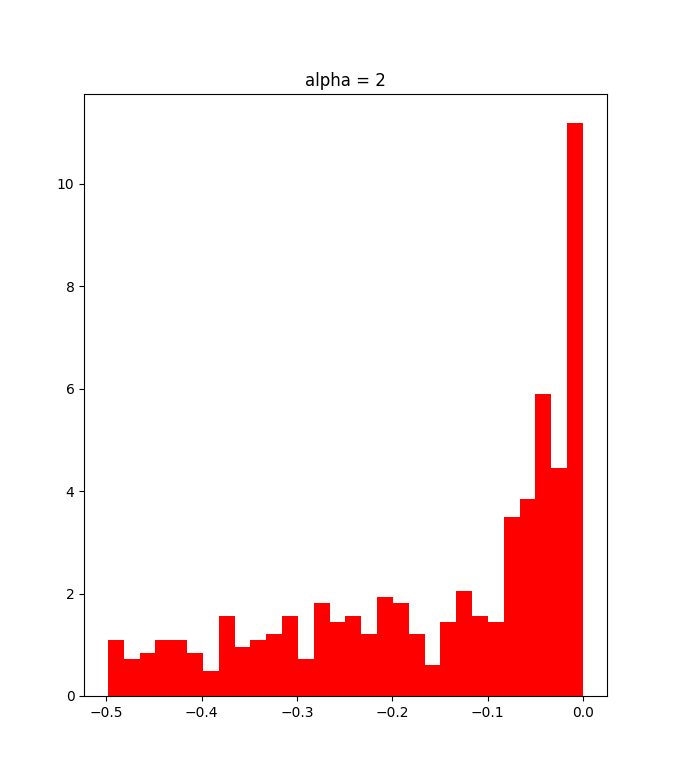
\includegraphics[width=80mm]{4_5.png}
\caption{Beta distrubution, alpha = 2}
\label{fig:example}
\end{figure}


\section*{Miniproject 4.3}

\begin{figure}[ht!]
\centering
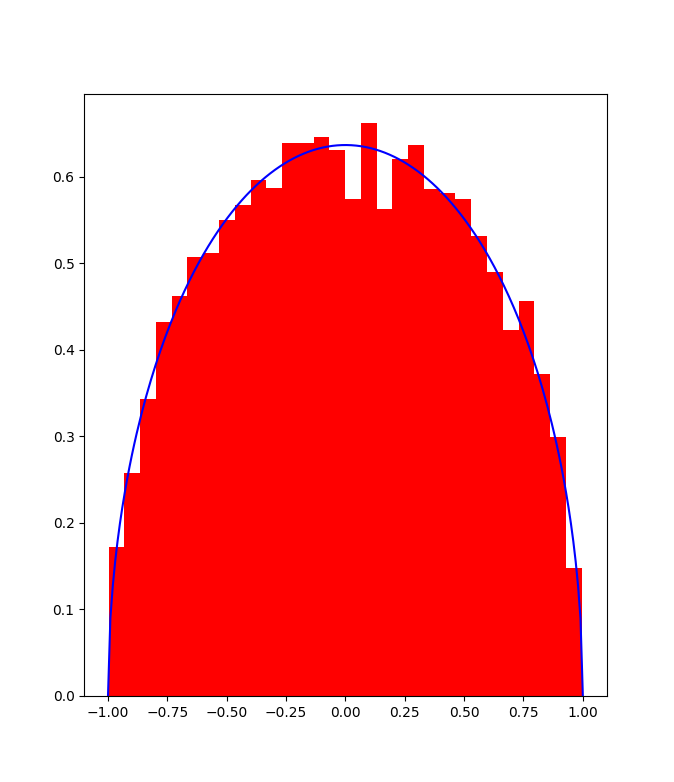
\includegraphics[width=80mm, height=50mm]{4_3.png}
\caption{Semi circular pde}
\label{fig:example}
\end{figure}

\newpage

\section*{Miniproject 5.3}

\begin{figure}[ht!] %add to template
\centering
\subfloat[]{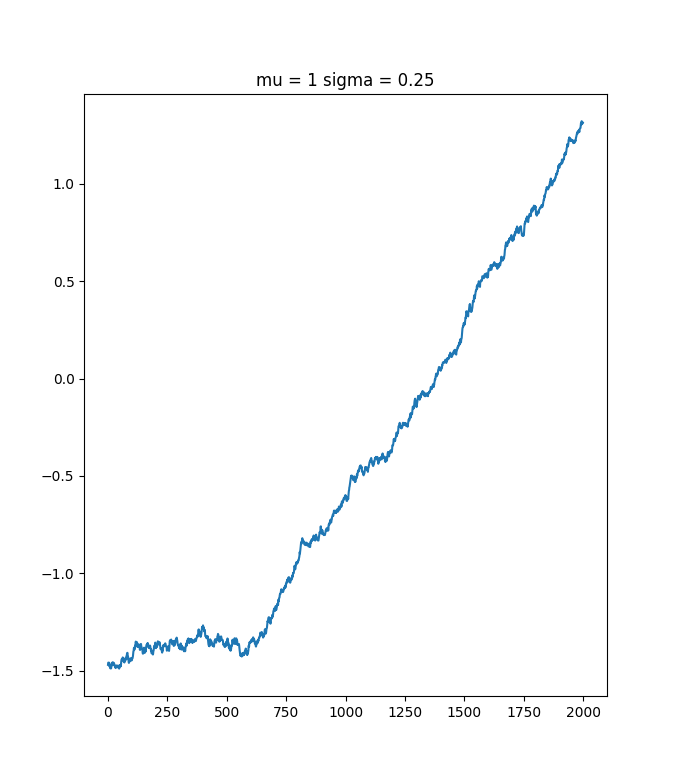
\includegraphics[width=70mm,height = 50mm]{5_3-1.PNG}}
\subfloat[]{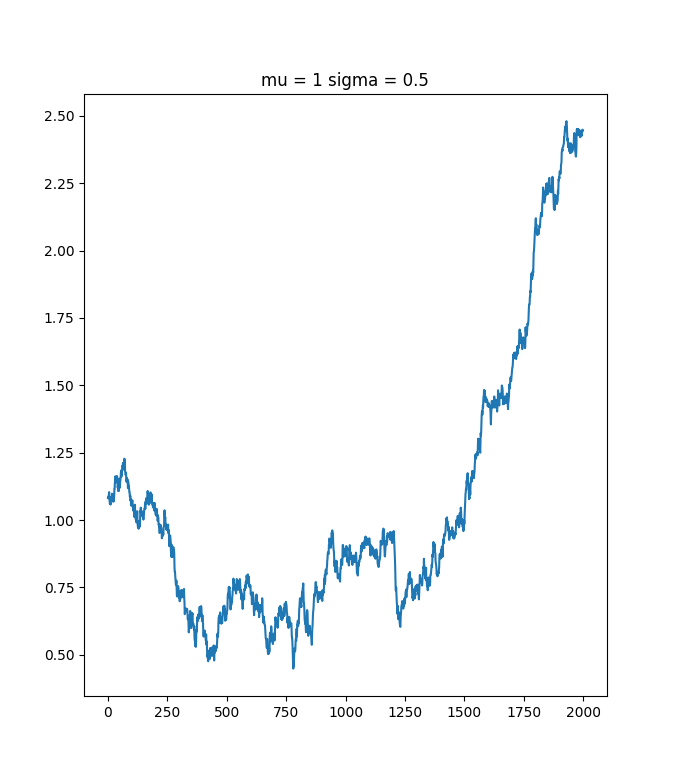
\includegraphics[width=70mm,height = 50mm]{5_3-2.PNG}}\\
\subfloat[]{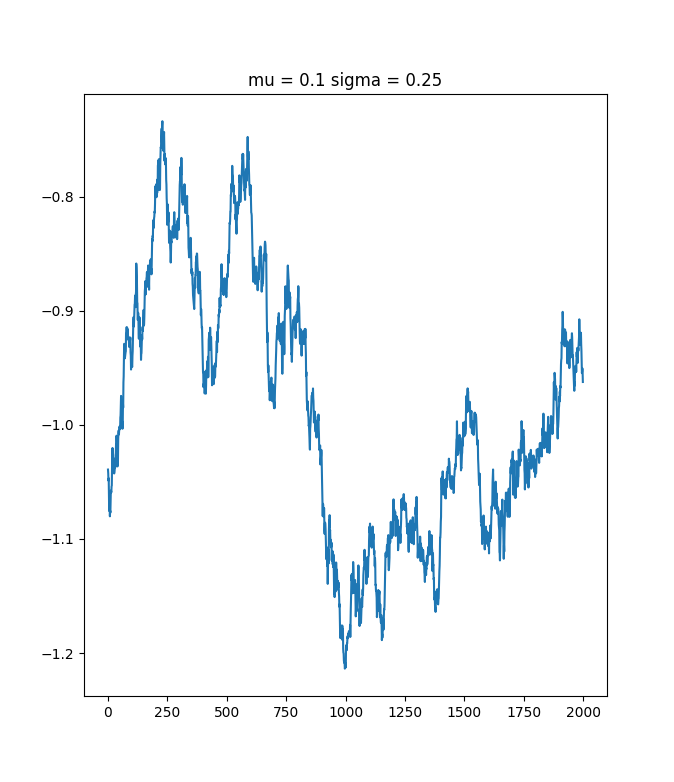
\includegraphics[width=70mm,height = 50mm]{5_3-3.PNG}}
\end{figure}

\section*{Miniproject 6.1}

\begin{itemize}
	\item \textbf{Output (N = 1000): } [14.2796957]
	\item \textbf{Output (N = 10000): } [12.41701961]
	\item \textbf{Output (N = 100000): } [11.9639898]
\end{itemize}


\section*{Miniproject 6.2}
\begin{itemize}
	\item \textbf{Output: }Approximation delta(0): [0.00041242]
	\item \textbf{Output: }Approximation delta(2): [3.1591858]
	\item \textbf{Output: }Approximation delta(4): [5.34118711]
\end{itemize}

\newpage
\section{Miniproject 7.1}
Calculate expected value of h($X_1*$, $X_2$) where h($x_1$,$x_2$) = $x_1x_2$. Changing the sum from X[0,:] to X[0,:]*X[1,:]).
\begin{lstlisting}[language=Python]
Hhat = np.zeros(4) 
for k in range(4):
	N = 10**(k+3) 
	X0 = [0,0] 
	X = McMcRandWalkGen(f, X0, Sigma, N) 
	Hhat[k] = 1/N*np.sum(X[0,:]*X[1,:])
print("MCMC estimates = ",np.round(Hhat,4))
\end{lstlisting}

\begin{itemize}
	\item \textbf{Output: } MCMC estimates =  [1.0904 1.1598 1.113  1.1292]
\end{itemize}

\bibliographystyle{unsrt}
\bibliography{references}
\end{document}